This report describes the development of the innovative mobile system for entertaining the visitors of the common social events such as concerts or exhibitions. The system comprises of two mobile applications, and it is titled Digital Lighter. This project is the part of the course TDT4290 Customer Driven Project. 
Customer Driven Project is held at The Norwegian University of Science and Technology accounted for 15 credits. The course aims to give the students a real experience with customers in a relevant IT project, and shall give the students a feel of managing a project in a group. The course will provide realistic experience in both report writing and product development driven by a customer. 

%\section{General information}
%This report is the delivery of this course, and it will be presented to an examiner at the end of the semester. It is also the most important part of the project, and it contains all the documentation for this project, everything from planning to the evaluation and conclusion. In the Table \ref{tab:structure_of_report} it is possible to see the structure, and the contents of this report. In the section belob it is also possible to read about the terminology for this report.

\section{Project purpose and concept}
The project was proposed by the consulting company Netlight represented by Peder Kongelf, who serves the role of the customer driving the project and communicating with the development team. Peder Kongelf together with company Netlight will be introduced in Section \ref{txt:introduction_stakeholders}.

The underlying task of this project is to develop the mobile application. The application will mainly be used as the mean to entertain the visitors of the music concerts, and other social events. This is allowing them to participate exclusively and share an experience by simply holding their mobile devices in the air. Each single visitor would for a short while become a pixel in the giant human screen made of the audience. 

The idea is based on the assumption that the overwhelming majority of people who would prospectively visit the concert posses a smartphone capable of running simple client application controlling the device's screen. At some point the whole audience would be instructed to raise their hands with the mobile devices' screens aimed towards the stage. The camera together with the big screen displaying the crowd would be placed on the stage so that the audience would be able to see their own reflection.

There would be another (server) application which would serve the purpose of controlling the camera, and detecting the audience devices. Once all of the devices are recognized, the server application would start sending the signals to each user device specifying which color it should display for the specified time frame. As a result it would be possible to display various imagery ranging from pictures to animations and videos on this big screen, which is consisting of visitors' smartphones aka pixels.

As the music concerts represent the events where people seeking for the enjoyment gather it is fairly easy to convince the visitors to join this shared experience. It can be widely seen now days that the concert managers, or even the musicians themselves are attempting to introduce specific added value to the concert by instructing the crowd to sing, dance or wave hands synchronously, in order to strengthen the whole musical experience. The satisfied visitors tend to visit the next event again, which is of course where the concert manager aims.

Therefore it can be said there is never enough of good and creative ideas about the crowd experience and joy catalyst. The Digital Lighter is one of them and as will be specified in Section \ref{sec:similar_projects} the market currently lacks such a product as this is truly innovative concept.

\section{Project name}
The customer wants a product to make the audience as a screen on a rock concert. 
The team has decided to name the product \emph{Digital Lighter}. 
This name was settled, because this product digitalizes the concept from "the old days", where the crowd at a concert held up lighters, to create a special atmosphere. 

\begin{figure}[hbt]
\centering
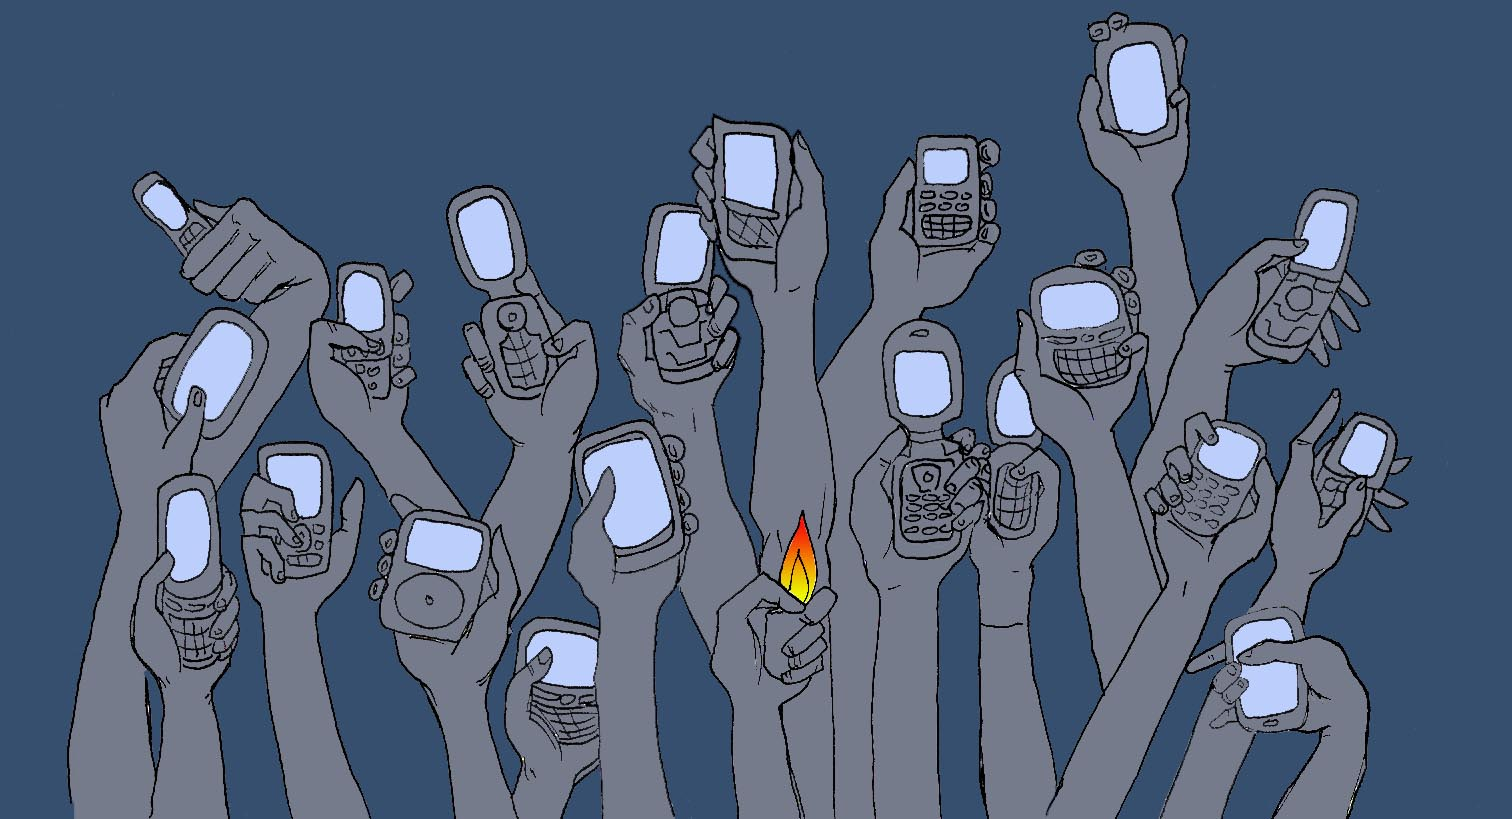
\includegraphics[width=\textwidth]{introduction/phones.jpg}
\caption{Digital Lighter}
\label{fig:digital lighter}
\end{figure}


\section{Goals}
Goals are statements that describe what the project will accomplish. 
The very first step in all projects is to define goals. 
It is important to spend sufficient time on this step, or else it can lead to unsuccessful project completion in many different ways. 
   
\label{sec:project-goals}

\subsection{Project goals}

\paragraph{Finish the project within the scheduled timetable}
One of the goals is to finish the project within the given time frame. 
In this particular case it means to deliver both product and report until 21th of November, when the final presentation take place.

\paragraph{Finish the project within the specified requirements}
Another goal is to make sure customer's needs described in requirements Chapter \ref{txt:requirements} are met.
This could be done simply by finishing the project with the specifics the customer really wanted. 
The best way to solidify this is to verify accomplishment by customer hand off and close down.

\subsection{Group goals}
\paragraph{Receive a good grade}
Getting a good grade is important because it says something about what you have learned in this course. 
This is relevant in terms of what job we might get when we have graduated. It also shows an employer that we can work hard. 
\paragraph{Receive a good recommendation from customer/supervisor}
If we work really hard, and impress the supervisor and the customer it would be nice to get a recommendation. This would be a bonus for our CV.

\subsection{Personal goals}
\paragraph{Agnethe}

My personal goal is to learn about group dynamics and collaboration. Another goal is to learn more about writing reports, because it is important to get some experience before writing for the masters degree. One of my goals is to deliver a product the customer is pleased with. It is also a great chance that I might work as an IT-consultant, and I want to learn as much as possible about this profession. I also want to learn as much as possible about android and mobile development. My last goal is to get better at holding presentations, because there will always be another presentation to hold. 

\paragraph{Jan}

This class was suggested to me by a few students who have already passed it. As from what I have learned it should be challenging and the students should receive a lot of experience while working on a project. From this point of view my personal goal is to improve my soft-skills regarding team collaboration as well as the technical skills, mostly the Java/Android programming. While I study at the Computer graphics department on my home university the image processing part of this project is also of the great value for me. I also expect to get the proper feedback from both the supervisor and the customer so I could learn from the mistakes or wrong approaches.

\paragraph{Milos}

I had the opportunity to work on actual projects before, but never as a part of a team. 
My primary goal is to determine how to cooperate and work with others in achieving mutual goals.
I want to learn about agile software development in practice.
To find out how to separate tasks, how to manage an ongoing project, and how to be a valuable part of the team.
I didn't expect to gain any technical knowledge of this course, but after discovering the project assignment I definitely want to learn about image processing.
I expected multicultural team and that report has to be written in English.
Therefore I wanted to profound my knowledge of English Language.

\paragraph{Tomas}
I have chosen NTNU university for my exchange studies because of this class. 
I was expecting to improve my soft-skills, software engineering knowledge and also my written and spoken English and to be treated like in real project.
As this class has already started, I can add to my personal goals also learning Java programming language,
Android platform development and improving my skills concerning image processing.

\section{Stakeholders} \label{txt:introduction_stakeholders}

The stakeholders in this project is any person or organization, which has some interest in, or is affected by this project. Together they construct the different restrictions and goals for the project. 
It is possible see the organization chart in Figure \ref{img:organization_chart}.

\begin{figure}[!ht]
    \begin{center}
    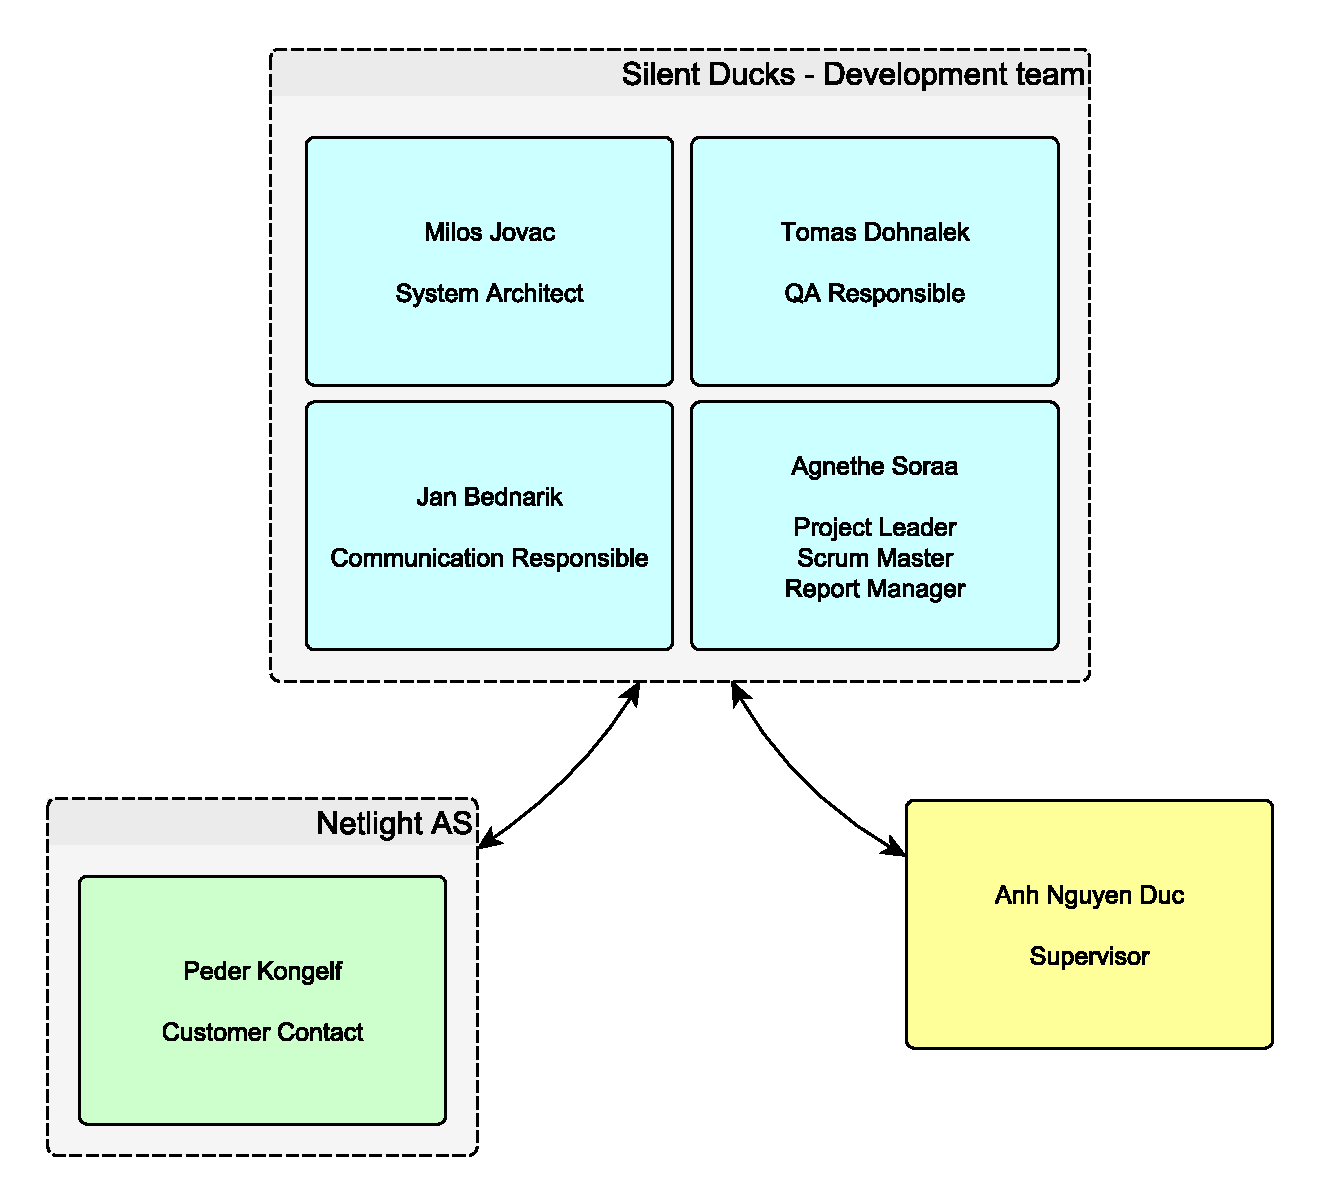
\includegraphics[width=12cm]{images/organization_chart.eps}
    \caption[Oganization chart]{Chart depicting team organization and its stakeholders}
    \label{img:organization_chart}
    \end{center}
\end{figure}

\paragraph{Customer}
Peder Kongelf is the customer. He works as an consultant for Netlight AS, which is a consulting company with field of expertise within IT management, IT governance, IT-strategy, IT-organization and IT-research. He has experiences with working as a consultant, working in scrum, and also with mobile development. He is able to provide the team guidance and support with various issues during the project, and even though he is the customer, he teaches the team a lot as well.      

 
\paragraph{Supervisor}
Anh Nguyen Duc is the supervisor assigned to this project. 
The main responsibility of the team's supervisor is to overview the whole project, discuss the work done, and also to discuss the future plans. 

Of course the interest from the university in general is to provide some real experience to the students, and prepare them for the business world.

\paragraph{Development team}
The development team's role is to meet all requirements presented by the customer and by The Department of Computer Science and Information Technology. 
The team is responsible for the development of the project, and the team is also responsible for writing all the documentation for this course.  



%\subsection{Stakeholder summary}
It is possible to see a list of stakeholders, with their contact information in Table \ref{tab:stakeholders_summary}.

\begin{table}[!ht]\centering
\caption{List of all stakeholders with their role and email contact}
\label{tab:stakeholders_summary}
\def\arraystretch{1.3}
\begin{tabular}{lll}
\toprule[0.5mm]
\textbf{Person} & \textbf{Email} & \textbf{Role}\\
\midrule
Peder Kongelf & peder.kongelf@gmail.com  & Customer\\
\midrule
Anh Nguyen Duc	 & anhn@idi.ntnu.no & Supervisor \\
\midrule
Milos Jovac &  milosjovac@gmail.com & Team member  \\
Jan Bednarik &  ja.bedna1@gmail.com & Team member\\
Agnethe Soraa & agnethes0raa@gmail.com & Team member  \\
Tomas Dohnalek & dohnto@gmail.com & Team member \\
\bottomrule[0.5mm]
\end{tabular}
\end{table}

\section{Structure of report}
It is possible to see the structure of this report in Table \ref{tab:structure_of_report}.
\begin{table*}[!ht]\centering
\caption{List of all chapters and short description}
\label{tab:structure_of_report}
\def\arraystretch{1.3}
\begin{tabularx}{\textwidth}{lX} \toprule[0.5mm]
\textbf{Chapter} & \textbf{Description} \\ \midrule
Chapter 1 & The \emph{introduction} chapter introduces the problem, and introduces the members and stakeholders of this project.
This chapter also explains the motivation and goals. \\

Chapter 2 &  The \emph{preliminary studies} chapter describes the work and research done. This chapter describes alternative approaches and solutions, and an evaluation of these. \\

Chapter 3 &  The \emph{planning} chapter describes the project plan, the organization, and planned workload.  \\

Chapter 4 &  The \emph{requirements} chapter describes the requirements, both functional and non-functional. It also describes use cases for the system. \\

Chapter 5	 &  The \emph{architecture} chapter explains the structure of the system, and how it is put together. \\

Chapter 6--12 	&  In the sprint chapters the reader can see how the product has developed during the time of the project. This includes planning, architecture, the implementation, testing and evaluation of the sprint. \\

Chapter 13 	 &  \emph{Evaluation} chapter includes the team dynamics and risk evaluation. Last but not least it describes an evaluation of the customer, supervisor and of course the task. \\

Chapter 14 	 &  \emph{Conclusion} chapter sums up the project, and discusses the solution, and looks at further work. \\

\midrule
Appendix 	 &   The appendix contains user manual, installation guide and examples of meeting minutes.\\

\bottomrule[0.5mm]
\end{tabularx}
\end{table*}

\section {Terminology}
\label{sec:terminology}
After a few meetings with the supervisor and customer, it was settled that terminology must be presented in report to prevent misunderstandings, especially since both customer and supervisor used different terminology.
Below there is listed product related terminology that will be used in further chapters of this report.

\paragraph{Client user}
is a participant of the concert who wants to actively take part in  the show, and is able to download the client application.

\paragraph{Server user}
or simply \textbf{Manager} is a person who controls what media should be played on the screen made from mobile phone's of users. 
The Server user can also manage other general settings.

\paragraph{End user} is either manager or end client user.

\paragraph{DigitalLighter}
is the final product. It is containing of two separate applications \emph{client} and \emph{server}.


\paragraph{Client} or \textbf{Client side} is an application controlled by client user, and provides an opportunity to be part of the screen by displaying figures on his mobile.

\paragraph{Server} or \textbf{Server side} is and application controlled by manager and provides an opportunity to change the media displayed on screen.

\paragraph{Pixel} is a client user's mobile phone under control of the manager.

\paragraph{Grid} is a matrix used as an abstraction for mapping mobile devices into a single pixel of an image.
The image of specific size requires the grid of specific suitable size.
For example imagine, that on the screen made of mobile devices, a single letter \emph{D} will be played.
This letter can be represented as an image displayed in Figure \ref{fig:grid_d} with size 4x4 pixels.
A grid is a 4x4 matrix created according to the image as shown in Figure \ref{fig:grid_mobiles}.

\begin{figure}[h]
        \centering
        \begin{subfigure}[b]{0.4\textwidth}
                
\includegraphics[width=\textwidth]{introduction/grid_d.png}
                \caption{Image to be displayed}
                \label{fig:grid_d}
        \end{subfigure}
        ~ %add desired spacing between images, e. g. ~, \quad, \qquad etc.
          %(or a blank line to force the subfigure onto a new line)
        \begin{subfigure}[b]{0.4\textwidth}
                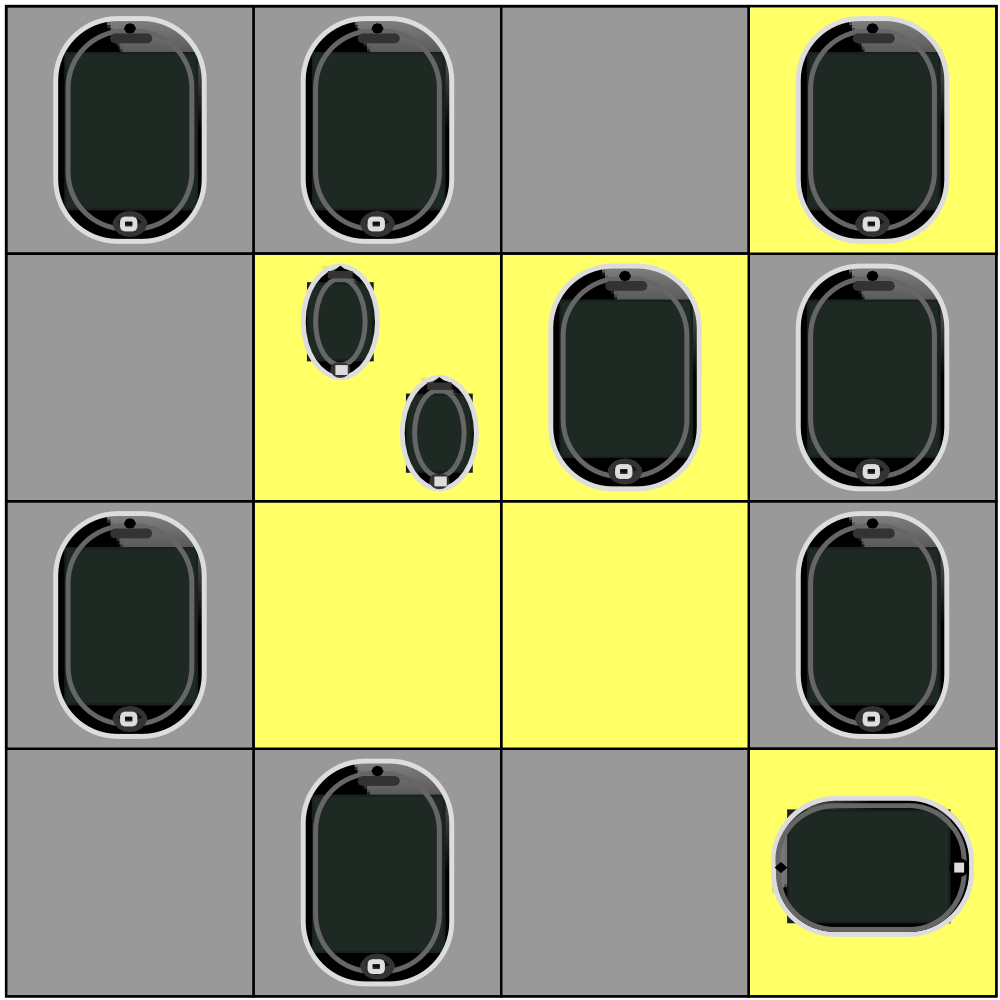
\includegraphics[width=\textwidth]{introduction/grid_mobiles.png}
                \caption{Appropriate grid with mobile devices}
                \label{fig:grid_mobiles}
        \end{subfigure}
        \caption{Grid example}\label{fig:grid}
\end{figure}